\subsection{Méthode \acrshort{AMDEC}}
\label{subsec:amdec}

L’\acrfull{AMDEC} constitue l’étape centrale de la sûreté de fonctionnement appliquée au projet SP-02. Elle permet de compléter
l’\acrlong{APR} et l’identification des \acrlong{MDF} en évaluant, pour chacun d’eux, la gravité potentielle de ses
conséquences, la fréquence d’apparition attendue et la capacité à les détecter au stade du développement ou à le maîtriser
avant qu’il ne produise un effet dangereux. L’objectif de cette démarche est:
\begin{enumerate}
    \item Quantifier la criticité de chaque mode de défaillance à l’aide d’indices normalisés (G, F, D) permettant de calculer
    l’\acrfull{IPR}.
    \item Prioriser les actions correctives en orientant les efforts de conception, de validation et d’essais vers les points du
    système les plus sensibles et les plus susceptibles de conduire à un \acrlong{ERP}.\\
\end{enumerate}

Dans le cadre du projet SP-02, l’\acrshort{AMDEC} s’applique aux sous-systèmes mécaniques, électroniques et logiciels, ainsi qu’aux
facteurs environnementaux. Cette approche permet d’évaluer non seulement les pannes, mais aussi leur impact dans des contextes
opérationnels variés, y compris en présence de combinaisons de défaillances, conformément à la règle ASF3 du \acrshort{CDC}
\gls{Fusex} bi-étage. L’\acrshort{AMDEC} présentée dans cette section s’appuie sur:
\begin{itemize}
    \item la liste des \acrfull{MDF} définis en section \ref{subsec:modes_deffaillance} ;
    \item les \acrfull{ERPs} identifiés en section \ref{subsec:analyse_prelem} ;
    \item la grille de cotation adoptée pour l’évaluation de la fréquence, de la gravité et de la détectabilité.\\
\end{itemize}

Elle constitue l’outil principal de justification de l’adéquation du design, des sécurités intégrées et du plan d’essais, en vue de
la validation finale présentée lors de la \acrshort{RCE}-3.\\

Pour réaliser cette analyse, nous devons d’abord définir une échelle pour les indices de gravité, de fréquence et de détectabilité
qui permettront ensuite de quantifier le risque de chaque \acrshort{MDF}:\\
\begin{itemize}
    \item Gravité (G) :
    \begin{enumerate}
        \item Effet négligeable / mission non compromise
        \item Effet mineur, intervention facile après vol
        \item Effet majeur partiel (réduction de performance / réparation nécessaire)
        \item Effet critique (dégâts importants, dégradation importante de la mission)
        \item Effet catastrophique (mise en danger des personnes, violation du gabarit, explosion)\\
    \end{enumerate}
    \item Fréquence (F)
    \begin{enumerate}
        \item Très rare (pratiquement impossible)
        \item Peu fréquent
        \item Probable occasionnellement
        \item Fréquent
        \item Très fréquent / tendance récurrente\\
    \end{enumerate}
    \item Détectabilité (D)
    \begin{enumerate}
        \item Très facile à détecter (contrôles simples détectent quasi systématiquement le problème)
        \item Facile à détecter (tests/indicateurs montrent généralement le problème)
        \item Moyennement détectable
        \item Difficilement détectable
        \item Très difficile à détecter avant l’événement (peu ou pas d’indications)\\
    \end{enumerate}
\end{itemize}

\newpage

Nous avons fait le choix d’utiliser le critère de détectabilité en tant que facteur diminuant la criticité d’un événement. Comme
elle réduit les scores, un \acrshort{MDF} facile à détecter apparaîtra moins critique que le même \acrshort{MDF} difficilement
détectable. La formule retenue pour le calcul de l’\acrshort{IPR} est donc la suivante: $IPR = G \times F \times \sqrt{D}$

\begin{figure}[h!]
    \centering
    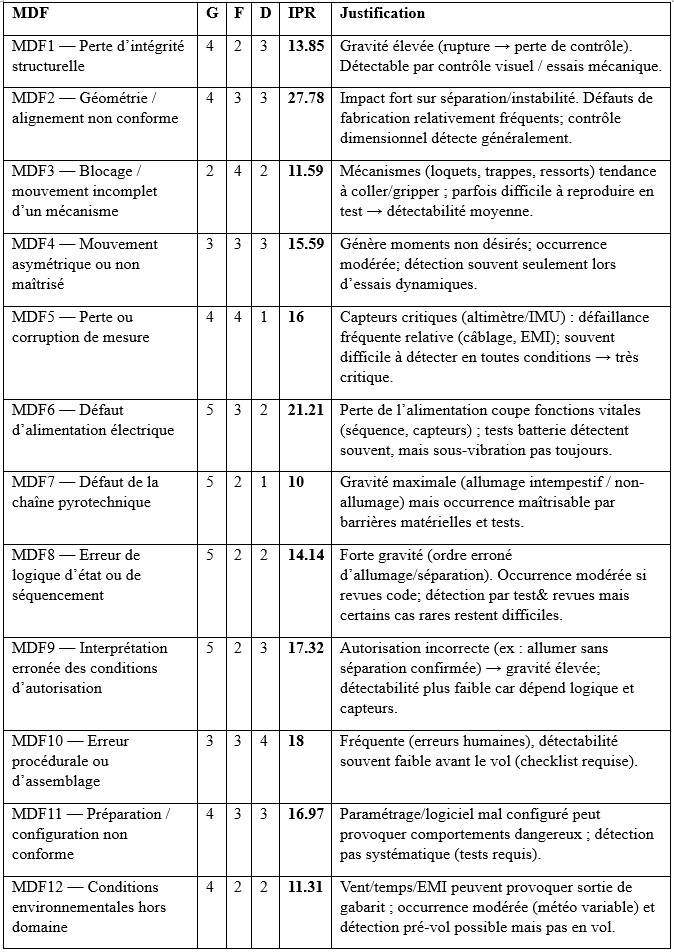
\includegraphics[width=0.85\textwidth]{figures/MDF_table_WORD.jpg}
    \caption{Tableau d'attribution des indices G, F, D et calcul de l'\acrshort{IPR} pour chaque \acrshort{MDF}}
\end{figure}

\newpage

La criticité permet de classer les modes de défaillance en fonction de leur gravité, de leur fréquence et de leur
détectabilité. Afin de faciliter l’analyse et de prioriser les actions correctives, des seuils indicatifs ont été définis. Ils
servent de guide pour distinguer les défaillances critiques nécessitant une action immédiate des défaillances moins
préoccupantes pouvant être simplement surveillées.\\

\begin{itemize}
    \item $IPR > 32$ — Niveau critique : défaillance majeure, inacceptable en l’état. Une action corrective ou une modification
    de conception est obligatoire avant la campagne de tir.
	\item $20 \le IPR \le 32$ — Niveau important : défaillance significative pouvant compromettre la mission. Une action
    corrective est nécessaire, soit par amélioration du design, soit par renforcement des procédures de contrôle.
	\item $12 \le IPR < 20$ — Niveau modéré : défaillance présente mais sous contrôle ; des mesures d’amélioration ou des
    tests supplémentaires sont recommandés pour réduire l’incertitude.
	\item $IPR < 12$ — Niveau faible : défaillance à faible impact ou bien maîtrisée ; aucune action immédiate n’est requise,
    mais une surveillance ou un contrôle ponctuel peut rester pertinent.
\end{itemize}

\begin{figure}[h!]
    \centering
    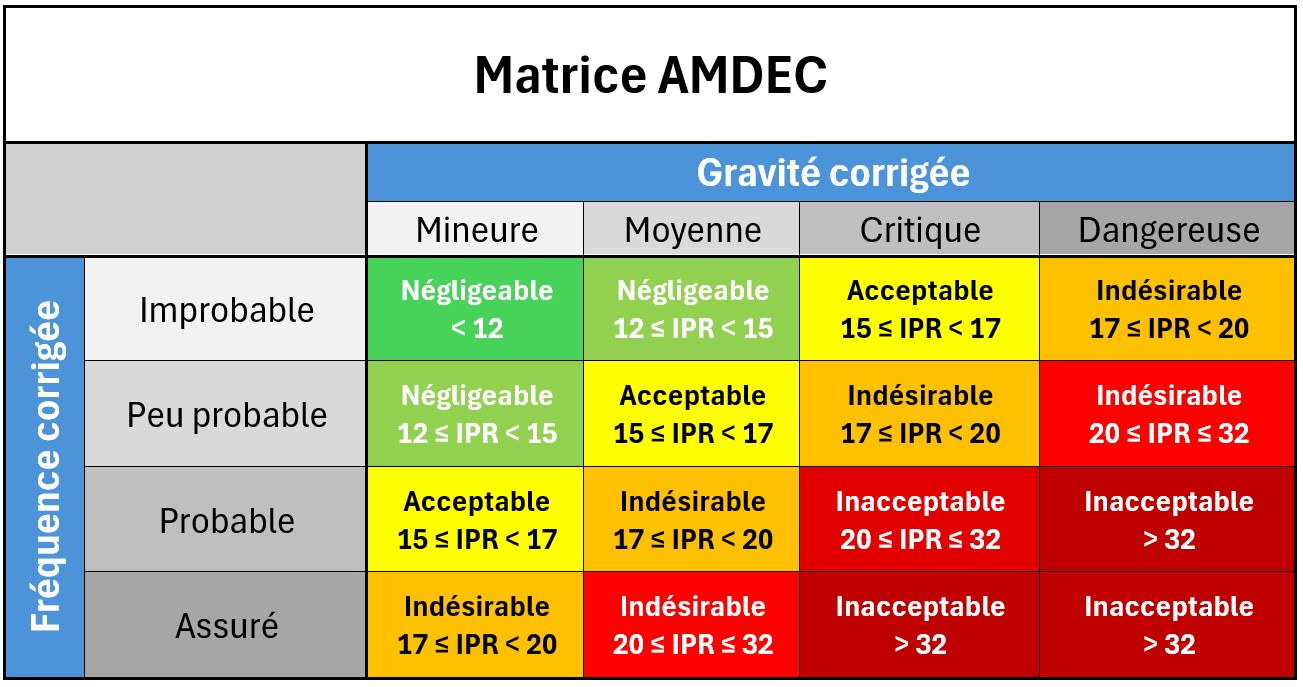
\includegraphics[width=\textwidth]{figures/AMDEC.jpg}
    \caption{Extrait de l'analyse \acrshort{AMDEC} réalisée pour le projet SP-02}
\end{figure}

\newpage
